%%%% Proceedings format for most of ACM conferences (with the exceptions listed below) and all ICPS volumes.
\documentclass[sigconf]{acmart}
%%%% As of March 2017, [siggraph] is no longer used. Please use sigconf (above) for SIGGRAPH conferences.

%%%% Proceedings format for SIGPLAN conferences 
% \documentclass[sigplan, anonymous, review]{acmart}

%%%% Proceedings format for SIGCHI conferences
% \documentclass[sigchi, review]{acmart}

%%%% To use the SIGCHI extended abstract template, please visit
% https://www.overleaf.com/read/zzzfqvkmrfzn


\usepackage{booktabs} % For formal tables
\usepackage{indentfirst}

% Copyright 
%\setcopyright{none}
%\setcopyright{acmcopyright}
%\setcopyright{acmlicensed}
\setcopyright{rightsretained}
%\setcopyright{usgov}
%\setcopyright{usgovmixed}
%\setcopyright{cagov}
%\setcopyright{cagovmixed}


% DOI
%\acmDOI{10.475/123_4}

% ISBN
%\acmISBN{123-4567-24-567/08/06}

%Conference
%\acmConference[WOODSTOCK'97]{ACM Woodstock conference}{July 1997}{El
  %Paso, Texas USA}
%\acmYear{1997}
%\copyrightyear{2016}


%\acmArticle{4}
%\acmPrice{15.00}

\begin{document}
\title{Temp Title: Non-Functional Bugs Project}
%\titlenote{Produces the permission block, and
  %copyright information}

\author{Aida Radu}
\affiliation{
  \institution{Dept. of Computing Science \\ University of Alberta}
  \city{Edmonton}
  \state{Canada}
}
\email{aradu@ualberta.ca}

\author{Sarah Nadi}
\affiliation{
  \institution{Dept. of Computing Science \\ University of Alberta}
  \city{Edmonton}
  \country{Canada}
}
\email{nadi@ualberta.ca}


\begin{abstract}
[PLACEHOLDER TEXT]

\end{abstract}

% The code below should be generated by the tool at
% http://dl.acm.org/ccs.cfm

\begin{CCSXML}
	<ccs2012>
	<concept>
	<concept_id>10011007</concept_id>
	<concept_desc>Software and its engineering</concept_desc>
	<concept_significance>500</concept_significance>
	</concept>
    
	<concept>
	<concept_id>10011007.10010940.10011003</concept_id>
	<concept_desc>Software and its engineering~Extra-functional properties</concept_desc>
	<concept_significance>500</concept_significance>
	</concept>
	</ccs2012>
\end{CCSXML}

\ccsdesc[500]{Software and its engineering}
\ccsdesc[500]{Software and its engineering~Extra-functional properties}


\keywords{Repository Mining; Bug Detection}


\maketitle

\section{Introduction}
\section{Background}
\section{Methodology}


To create our dataset, we looked at a variety of Github repositories written in either java or python. 


\subsection {Project selection}
We used two main methods to identify candidate repositories for mining. 
First, we used the Github API to search for projects written in java or python, and sorted them based on their number of stars. We found several instances where developers corrected memory leaks, or replaced one API with another to improve performance. Thus, for our second method we identified candidate repos using Github`s search bar find similar changes. We searched for commits containing keywords such as ``StringBuilder replace,'' ``foreach loop replace,'' and ``fix memory leak.''


\subsection{Obtaining commits}
To extract commits related to non-functional requirements, we implemented a keyword search using PyDriller \footnote{https://github.com/ishepard/pydriller, Davide Spadini 2018}. The stemmed keywords are listed in Table 1. Example word endings are in square brackets.

% ----------------------------------- WIP -------------------------------------------------
\begin{table}

  \caption{Commit Message Keywords}
  \label{tab:kwds}
\begin{tabular}{  c c c }
\toprule
 "fix"&"bug"&"error"\\
 "refactor"&"secur[ity]" &"maint[enance]"\\
 "stab[ility]"&"portab[ility]"&"efficien[cy]"\\
 "usab[ility]" & "reliab[ility]"&"testab[ility]"\\
 "changeab[ility]"& "replace"&"memory"\\
 "resource"& "runtime"&"crash"\\
 "leak" &"attack" &"authenticat[ion]"\\
 "authoriz]ation]"& "cipher"&"crack" \\ 
 "decrypt"&"encrypt"&"vulnerab[ility]"\\ 
 "minimize"&"optimize"&"slow"\\
 "\#"& &\\
\bottomrule
\end{tabular}
\end{table}

%--------------------------------------------------------------------------------------------------


For those repositories identified by star rating, we directly ran PyDriller; note that some of these projects contained zero true positives. For projects identified via the Github search, we first documented the bug that was initially found in the search, then ran the PyDriller program on the complete repo history. Thus, these projects always had at least one true positive. 

Our PyDriller program mined the commit history of each project, and outputted a CSV file containing the id and message of the commits containing one or more of the keywords in Table 1. For projects written in Java, we further limited our search to commits affecting \texttt{.java} files. Likewise, for python projects, we looked at \texttt{.py} files.

We then manually searched these files for true positives. We ignored commits that, despite containing one or more of the keywords in our list, did not relate to non-functional requirements (e.g., ``Fix copy paste error''\footnote{https://github.com/jenkinsci/jenkins/commit/9fb6ccf} and ``Allow modules to replace visual character representation''\footnote{https://github.com/MovingBlocks/Terasology/commit/45f915a}). 

\subsection{Documentation}
For each problem we identified, we recorded the problem meta data in a YAML\footnote{http://yaml.org/, last checked on June 27, 2018} file. Figure 1 shows an example of our format. Each file contains the problem's \texttt{commit url} and \texttt{commit message}, as well as the particular \texttt{file} and \texttt{method} where developers made the fix. Because a user`s commit message is not always thorough, we explained our interpretation of the problem under a \texttt{description} field. For fixes related to specific APIs (e.g., using a StringBuilder in place of  a String), we recorded the involved \texttt{API}, as well as a \texttt{rule} corresponding to the change. For commits not connected to a particular API, we created a general \texttt{suggestion} to address similar problems.

\begin{figure}
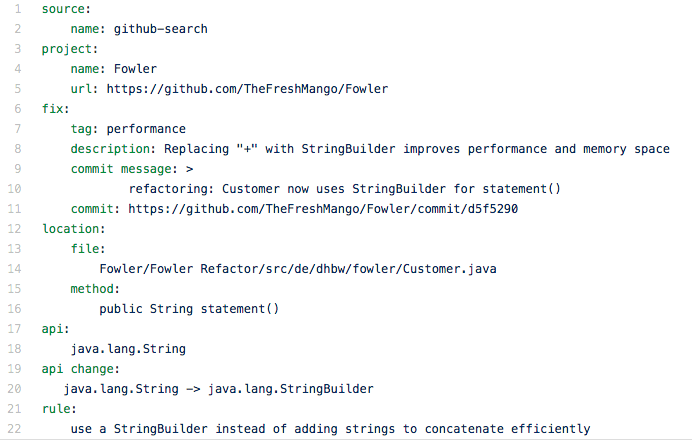
\includegraphics[height=2in, width=3in]{YAMLmetadata}
\caption{Meta Data for \texttt{Fowler} - problem 2}
\end{figure}


\section{Dataset}
\section{Discussion and Directions for Future Work}
\section{Conclusions}
\section*{threats to validity}


\section*{Acknowledgements}


\bibliographystyle{ACM-Reference-Format}
\bibliography{bibRaduNadi2018}

\end{document}
